% SPDX-License-Identifier: CC-BY-SA-4.0
% Author: Matthieu Perrin
% Part: <Nom de la partie>
% Section: <Nom de la section>
% Sub-section: <Nom de la sous-section>  % (facultatif, laisser vide si non utilisé)
% Frame: <Titre de la slide>

\begingroup

\begin{frame}{Classes de complexité importantes}

  \begin{block}{Classes de complexité \alert{non-déterministe} importantes}

    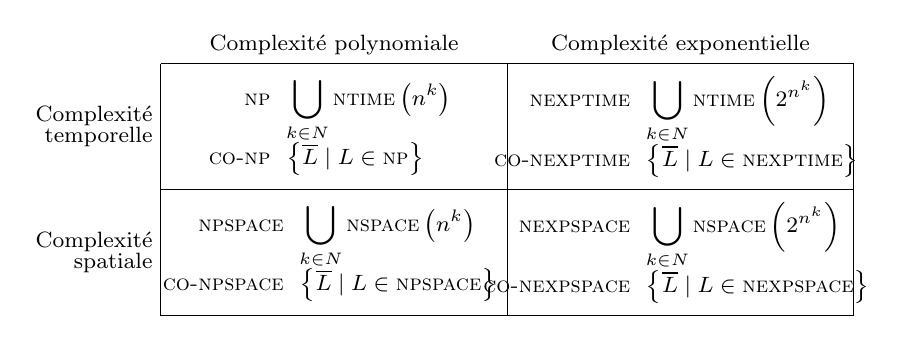
\begin{tikzpicture}[y=8mm, x=22mm]\footnotesize
      \draw (0,0) -- (4,0);
      \draw (0,2) -- (4,2);
      \draw (0,4) -- (4,4);
      \draw (0, 0) -- (0, 4);
      \draw (2, 0) -- (2, 4);
      \draw (4, 0) -- (4, 4);
      
      \node[align=center] at (1,3) {
        $\begin{array}{@{}r@{~}c@{~}l@{}}
          \alert{\textsc{np}} & \alert{\eqdef} & \displaystyle\alert{\bigcup_{k\in \mathbb{N}} \textsc{ntime}\left(n^k\right)}\\
          \textsc{co-np} & \eqdef & \left\{ \overline{L} \mid L \in \textsc{np} \right\}
        \end{array}$
      };
      \node[align=center] at (3,3) {
        $\begin{array}{@{}r@{~}c@{~}l@{}}
          \alert{\textsc{nexptime}} & \alert{\eqdef} & \displaystyle \alert{\bigcup_{k\in \mathbb{N}} \textsc{ntime}\left(2^{n^k}\right)}\\
          \textsc{co-nexptime} & \eqdef & \left\{ \overline{L} \mid L \in \textsc{nexptime} \right\}
        \end{array}$
      };
      \node[align=center] at (1,1) {
        $\begin{array}{@{}r@{~}c@{~}l@{}}
          \alert{\textsc{npspace}} & \alert{\eqdef} & \displaystyle\alert{\bigcup_{k\in \mathbb{N}} \textsc{nspace}\left(n^k\right)}\\
          \textsc{co-npspace} & \eqdef & \left\{ \overline{L} \mid L \in \textsc{npspace} \right\}
        \end{array}$
      };
      \node[align=center] at (3,1) {
        $\begin{array}{@{}r@{~}c@{~}l@{}}
          \alert{\textsc{nexpspace}} & \alert{\eqdef} & \displaystyle \alert{\bigcup_{k\in \mathbb{N}} \textsc{nspace}\left(2^{n^k}\right)}\\
          \textsc{co-nexpspace} & \eqdef & \left\{ \overline{L} \mid L \in \textsc{nexpspace} \right\}
        \end{array}$
      };
      \node[align=center, above] at (1,4) {Complexité \structure{polynomiale}};
      \node[align=center, above] at (3,4) {Complexité \structure{exponentielle}};
      \node[align=right,  left ] at (0,1) {Complexité\\[-2pt]\structure{spatiale}};
      \node[align=right,  left ] at (0,3) {Complexité\\[-2pt]\structure{temporelle}};
    \end{tikzpicture}
  \end{block}

  \structure{Remarque :} classes stables pour les extensions du modèle de MTND

  \begin{exampleblock}{Exemple -- Le problème \textsc{Subset-Sum}}
    \begin{itemize}
    \item On a une MTND étendue qui reconnaît \textsc{Subset-Sum} en temps linéaire
    \item Donc il y a une MTND stricte qui reconnaît \textsc{Subset-Sum} en temps $\textsc{poly}$
    \item Donc \example{$\textsc{Subset-Sum} \in \textsc{np}$}
    \end{itemize}
  \end{exampleblock}
  
\end{frame}

\endgroup
